

%----------------------------------------------------------------------------------------
%	PACKAGES AND OTHER DOCUMENT CONFIGURATIONS
%----------------------------------------------------------------------------------------

\documentclass[a0,portrait]{a0poster}

\usepackage{multicol} % This is so we can have multiple columns of text side-by-side
\columnsep=50pt % This is the amount of white space between the columns in the poster
\columnseprule=0pt % This is the thickness of the black line between the columns in the poster

\usepackage[svgnames]{xcolor} % Specify colors by their 'svgnames', for a full list of all colors available see here: http://www.latextemplates.com/svgnames-colors

\usepackage{times} % Use the times font
%\usepackage{palatino} % Uncomment to use the Palatino font

\graphicspath{{figures/}} % Location of the graphics files
\usepackage{booktabs} % Top and bottom rules for table
\usepackage[font=small,labelfont=bf]{caption} % Required for specifying captions to tables and figures
\usepackage{amsfonts, amsmath, amsthm, amssymb} % For math fonts, symbols and environments
\usepackage{wrapfig} % Allows wrapping text around tables and figures
% \usepackage[labelformat=empty]{caption}
\usepackage{fontawesome}
\usepackage[utf8]{inputenc}
\usepackage{url}
\usepackage{graphicx}
\usepackage{geometry}
\addtolength{\textwidth}{20cm}
\geometry{margin=5cm, rmargin=5cm, marginparwidth=0cm}
\begin{document}

%----------------------------------------------------------------------------------------
%	POSTER HEADER 
%----------------------------------------------------------------------------------------

% The header is divided into two boxes:
% The first is 75% wide and houses the title, subtitle, names, university/organization and contact information
% The second is 25% wide and houses a logo for your university/organization or a photo of you
% The widths of these boxes can be easily edited to accommodate your content as you see fit

\begin{minipage}[b]{0.75\linewidth}
\VeryHuge \color{NavyBlue} \textbf{Evaluating dengue forecasting models to 
predict Zika and Chikungunya in Brazil.}
\color{Black}\\[0.4cm] 
\Large \textbf{
\authorName{Flávio Codeço Coelho}{1\space\Letter}, 
\authorName{Elisa Mussumeci}{1}, 
%\authorName{N.~Gustafsson}{1}, 
\authorName{Marcelo Orgler}{1}, 
\authorName{Linneu Holanda}{1}} 
% Author(s)
\\
\vspace{1cm}
\large \textbf{
\authorAffil{1}{Fundação Getulio Vargas, Brazil}; 
\large \textbf{Correspondence to: fccoelho@fgv.br}}
\begin{center}
    \large \textbf{Poster DOI: ADD here from figshare \\ \faGithub \ 
github.com/AlertaDengue | \faTwitter \ @fccoelho}
\end{center}
\end{minipage}
%
\begin{minipage}[b]{0.25\linewidth}
\begin{center}

\includegraphics[width=15cm]{figures/Marca_FGV_EMAp.png}\\ 

\includegraphics[width=16cm]{figures/geomed.png}\\
\end{center}
\end{minipage}

%\vspace{.2cm} % A bit of extra whitespace between the header and poster content

%----------------------------------------------------------------------------------------

\begin{multicols}{3} % This is how many columns your poster will be broken into, a portrait poster is generally split into 2 columns

%----------------------------------------------------------------------------------------
%	ABSTRACT
%----------------------------------------------------------------------------------------

\noindent
The Mosquito Aedes aegypti is a vector for multiple viruses around the globe. 
Its distribution is restricted to tropical and subtropical climates, which 
reflects its sensitivity to temperature, humidity and other weather constraints. 
The modulation of its life cicle by climate, shapes the seasonality of the 
diseases it transmits. 
 In Brazil, Aedes aegypti has been mainly associated with the transmission of 
dengue, making it a marked seasonal disease. In recent years, A. aegypti has 
also been notably responsible for epidemics of the Zika and Chikungunya virus. 
In this paper we explore the performance of dengue forecast models trained on 
the longer available incidence timeseries to predict the weekly incidence of 
Zika and Chikungunya as well.  We will use a LSTM (long short term memory) 
recursive neural network model, which we have shown, in a previous work, to 
yield accurate forecasts for weekly dengue incidence. We will also compare it 
to a Random Quantile Forest model. Climate variables such as temperature, 
humidity, and atmospheric pressure are also used as predictors. A spatial 
component built from the incidence at neighboring cities is also included. We 
present results of the forecast of total incidence of arboviral disease as well 
as of each disease separately and discuss the relative performances of the model 
for each of these tasks.

\begin{center}
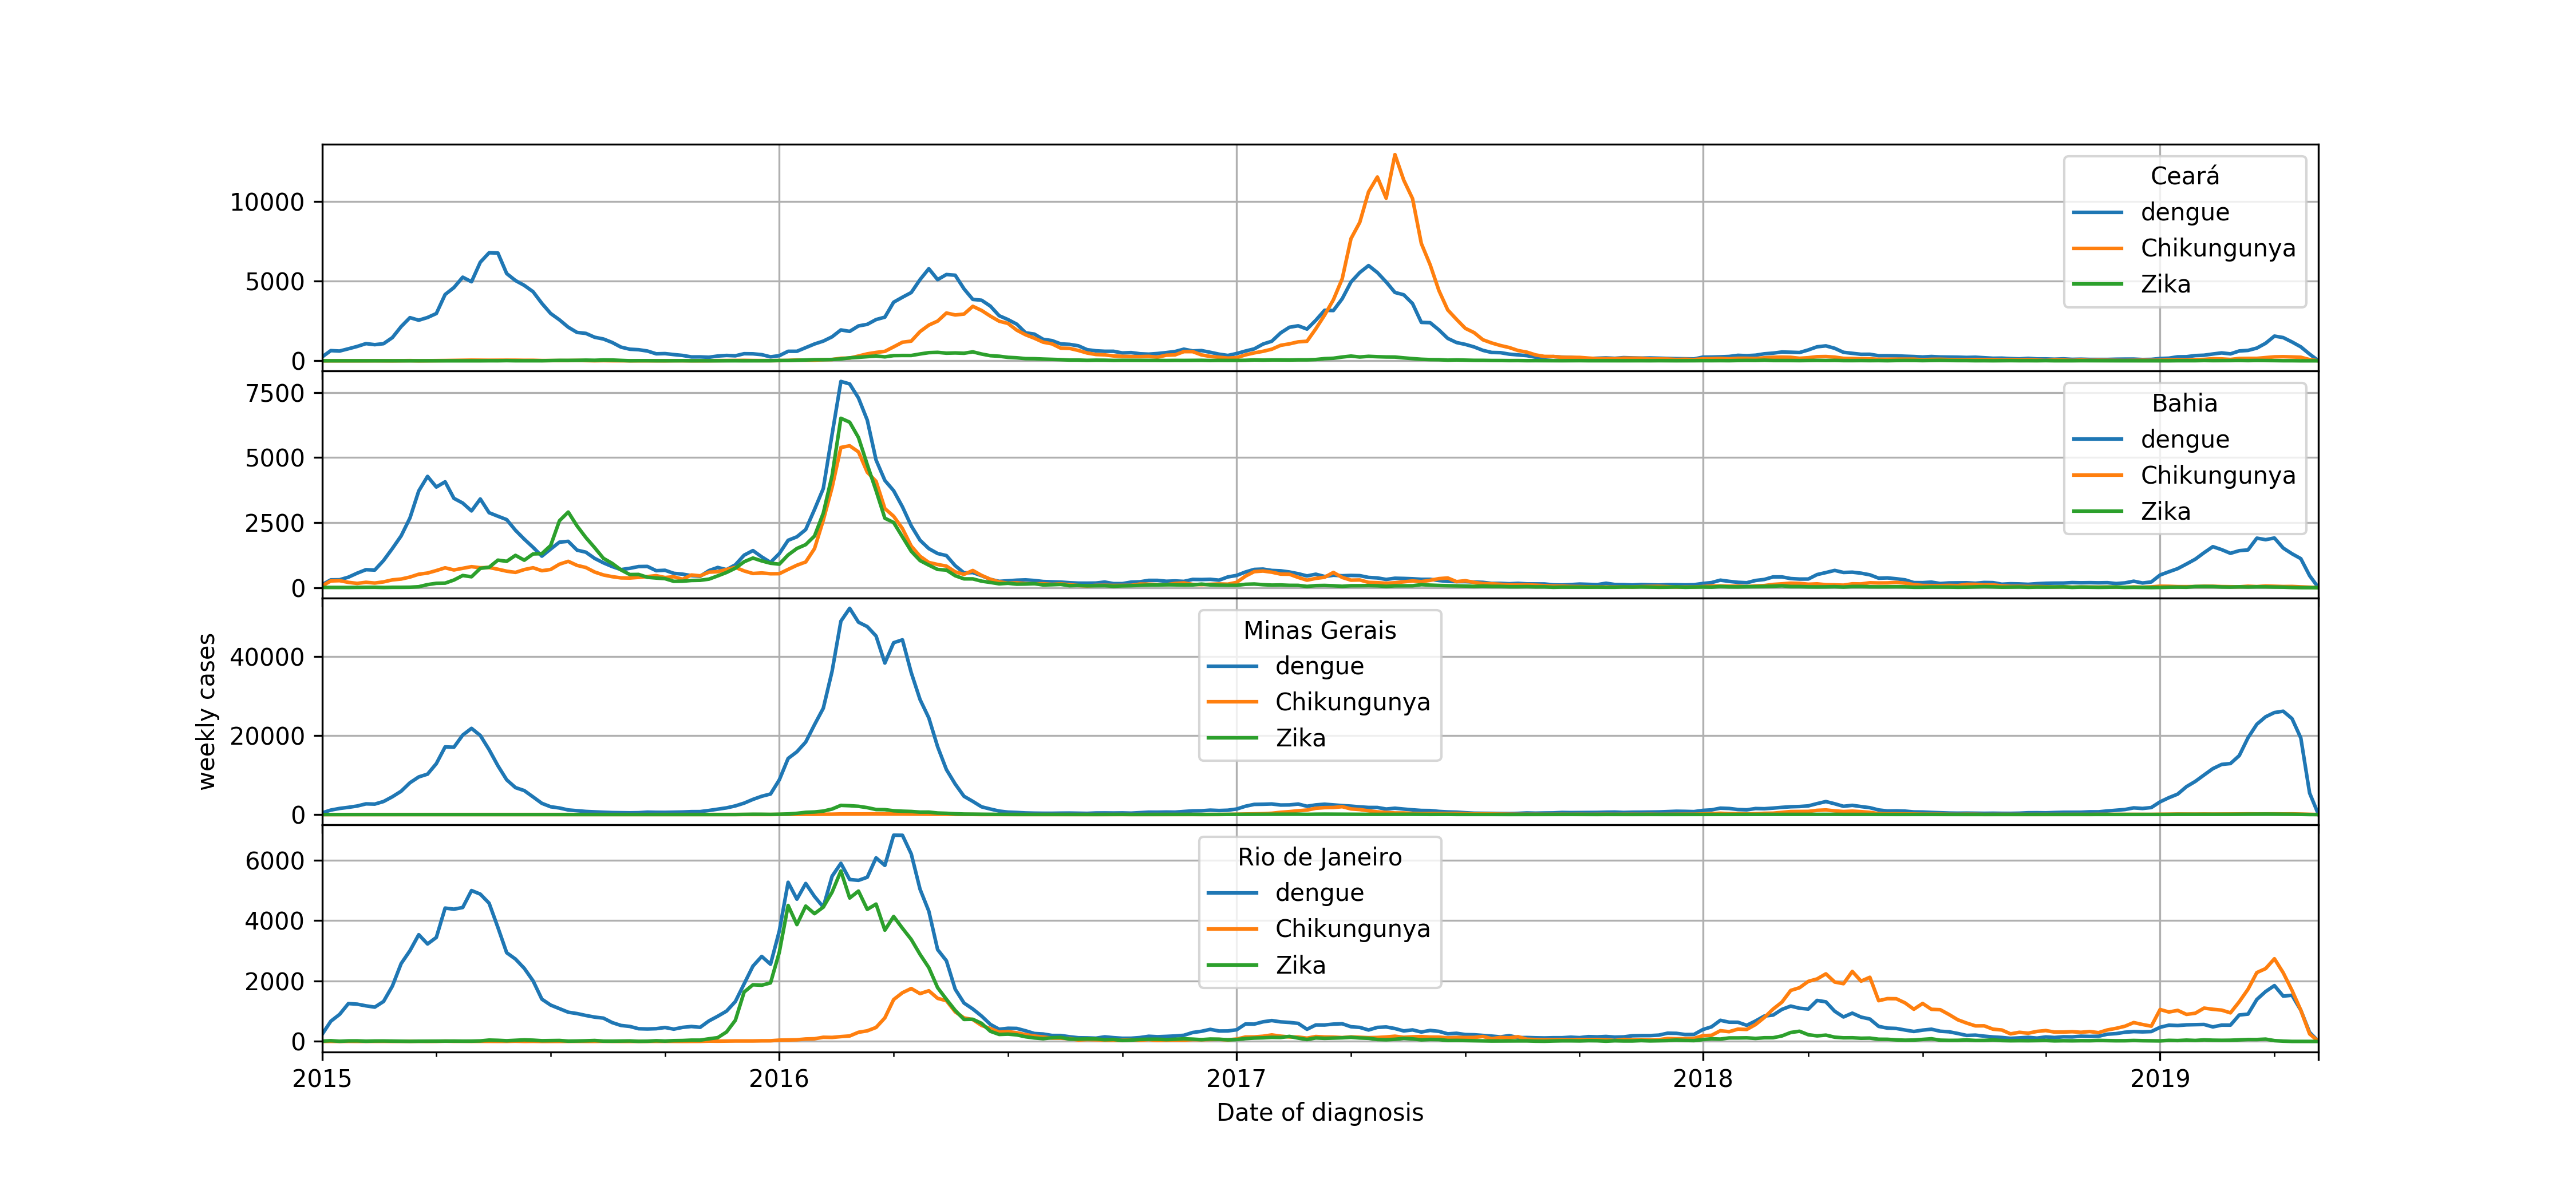
\includegraphics[width=\linewidth]{figures/dcz_series.png}
\captionof{figure}{\textbf{Weekly incidence for the state of Ceará, Brazil.} 
The three arboviroses incidences are correlated.}
\label{fig:series}
\end{center}%\vspace{1cm}

The data used in this work comes from the Infodengue project, which monitors 
these arboviroses in Brazil. In figure \ref{fig:series} we can see the 
incidence series for states in Brazil which had significant outbreaks of the 3 
arboviroses since 2016 when Chikungunya and Zika arrived in Brazil.


\section*{Dengue forecast models}
Both LSTM and RQF models were trained to predict 4 weeks ahead of the last data 
point($w_{t+4}$). Both models use 4 weeks of historical data to generate 
forecasts. Forecasts are done in a rolling window fashion. Both models use as 
predictors, the following series: number of cases, Effective reproduction 
number ($R_t$),Temperature, Humidity and Atmospheric pressure.
\paragraph*{LSTM.}
A LSTM model is a recurrent deep neural network model developed to handle 
predictions of timeseries. We used a LSTM model with 3 LSTM units followed by 
3 dropout layers. The model was trained for 300 epochs using a mean-log 
squared-error (MLSE) loss function  and a Nesterov Adam 
optimizer\cite{sutskever2013importance}. Figure \ref{fig:dengue_LSTM} shows 
dengue forecasts by the LSTM model for Fortaleza.

\begin{center}
    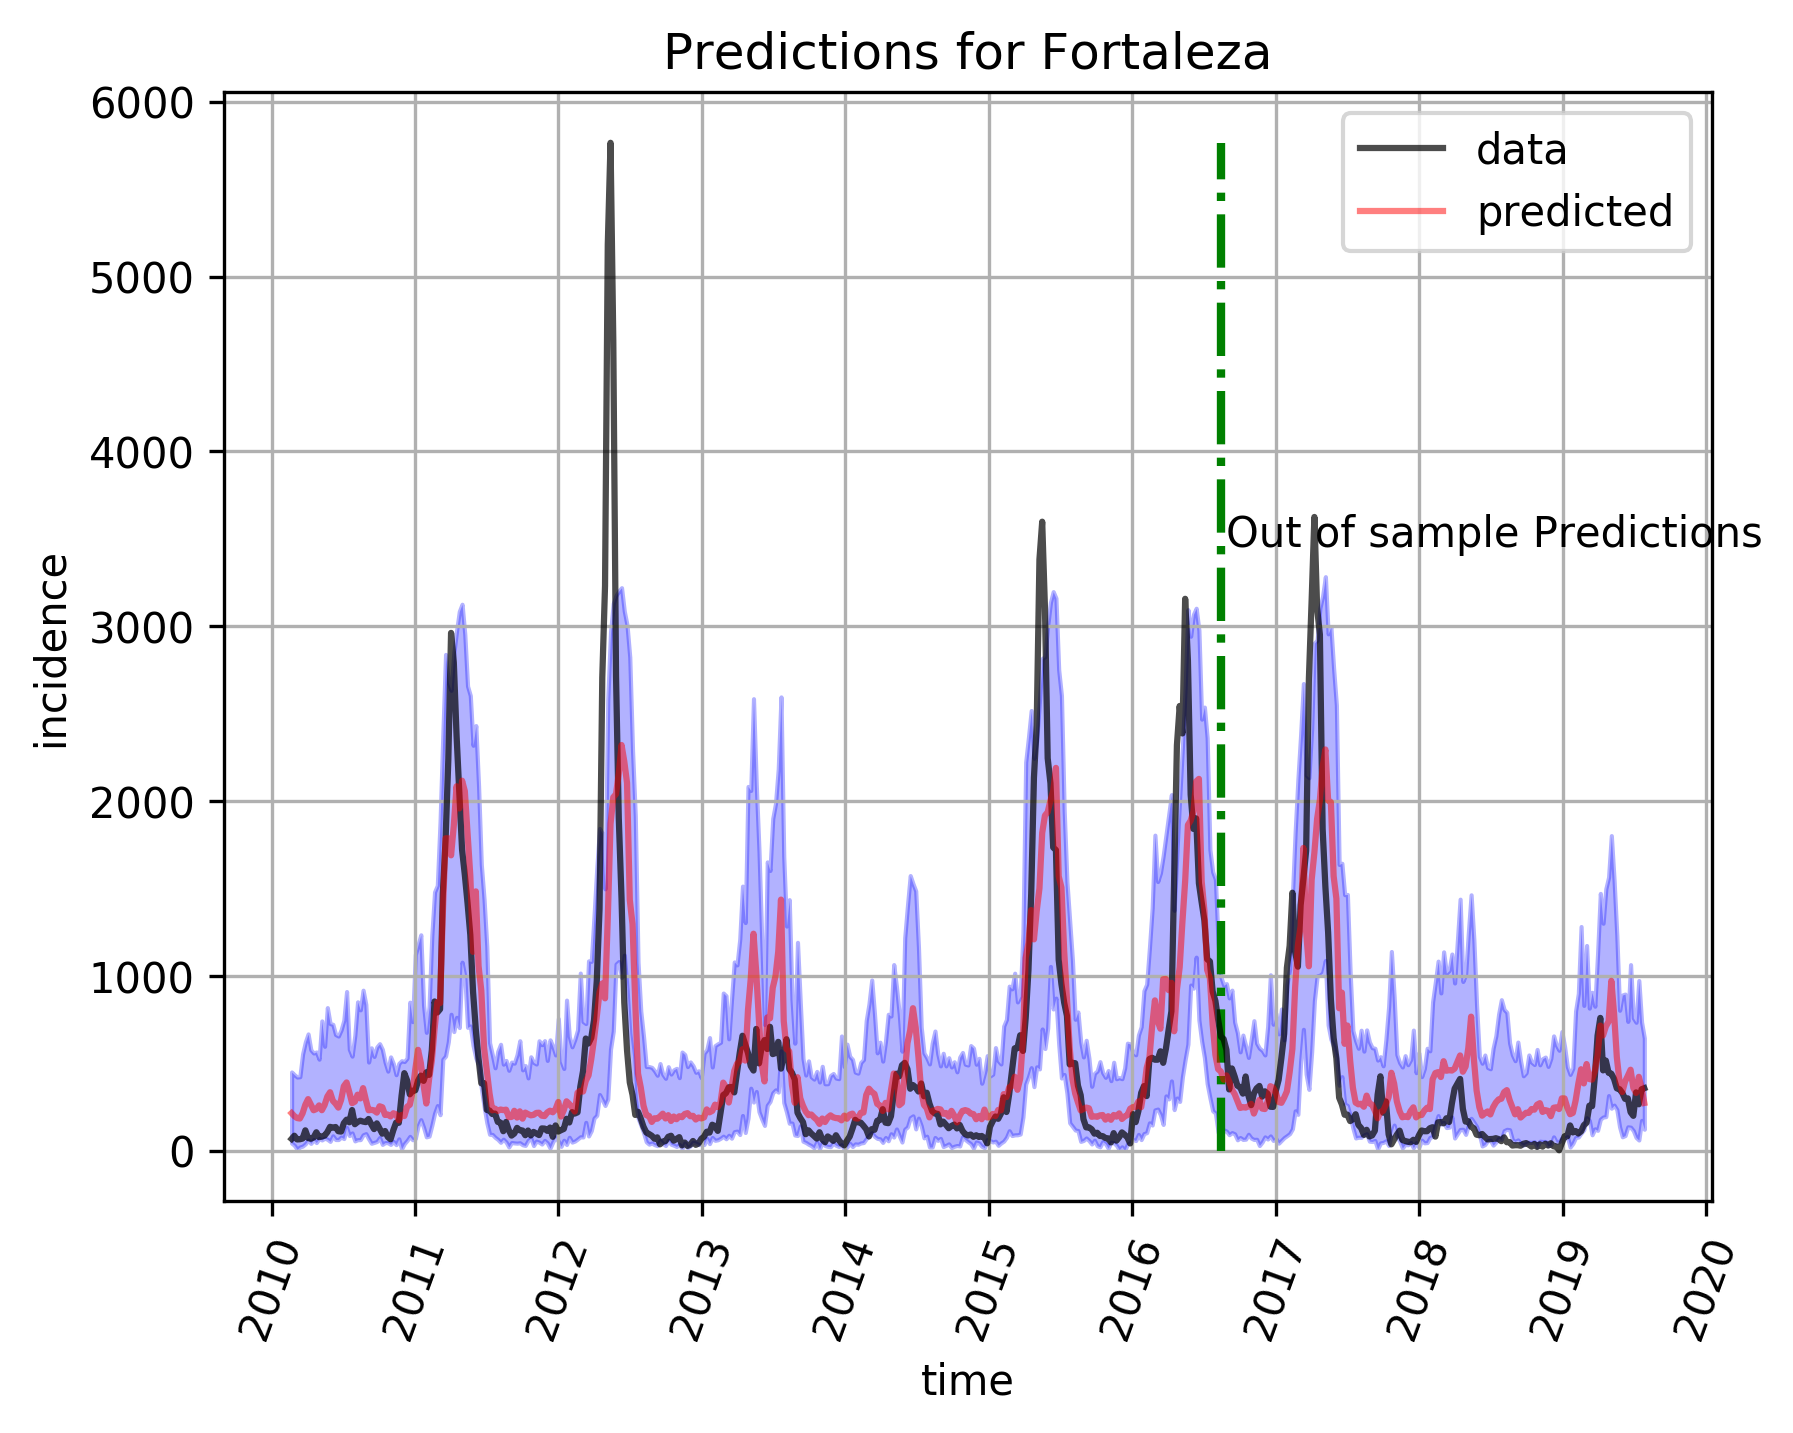
\includegraphics[width=0.8\linewidth]{figures/lstm_Fortaleza_unc.png}
    \captionof{figure}{\textbf{LSTM forecast for Dengue incidence (black line)} 
Prediction (red line) with 95\% interval for the city of Fortaleza. Every point 
in the red 
line corresponds to prediction from 4 weeks before.}\label{fig:dengue_LSTM}
\end{center}%\vspace{1cm}

\paragraph*{Random Quantile Forest (RQF).}
Random Forest models calculate an ensemble of regression trees from random 
subsets of data. RQF models are an extension to regular random forests in which 
the full conditional distribution of $Y$ given $X=x$ is calculated. As a 
result, it is a non-parametric, consistent and accurate way to determine 
conditional quantiles from high-dimensional 
predictors\cite{meinshausen2006quantile}. Let $T$ be an array containing the 
${\mathcal D=4}$ most recent observations from each 
series in the predictor matrix. Thus the regression model can be simply 
represented by
\begin{equation}
\hat{y}_{t+\tau} = \beta_{t} T_{t} + \epsilon_t
\label{eq:rf_trans}
\end{equation} 

Figure \ref{fig:dengue_RQF} shows dengue forecasts for Rio de Janeiro by the 
RQF model.

\begin{center}
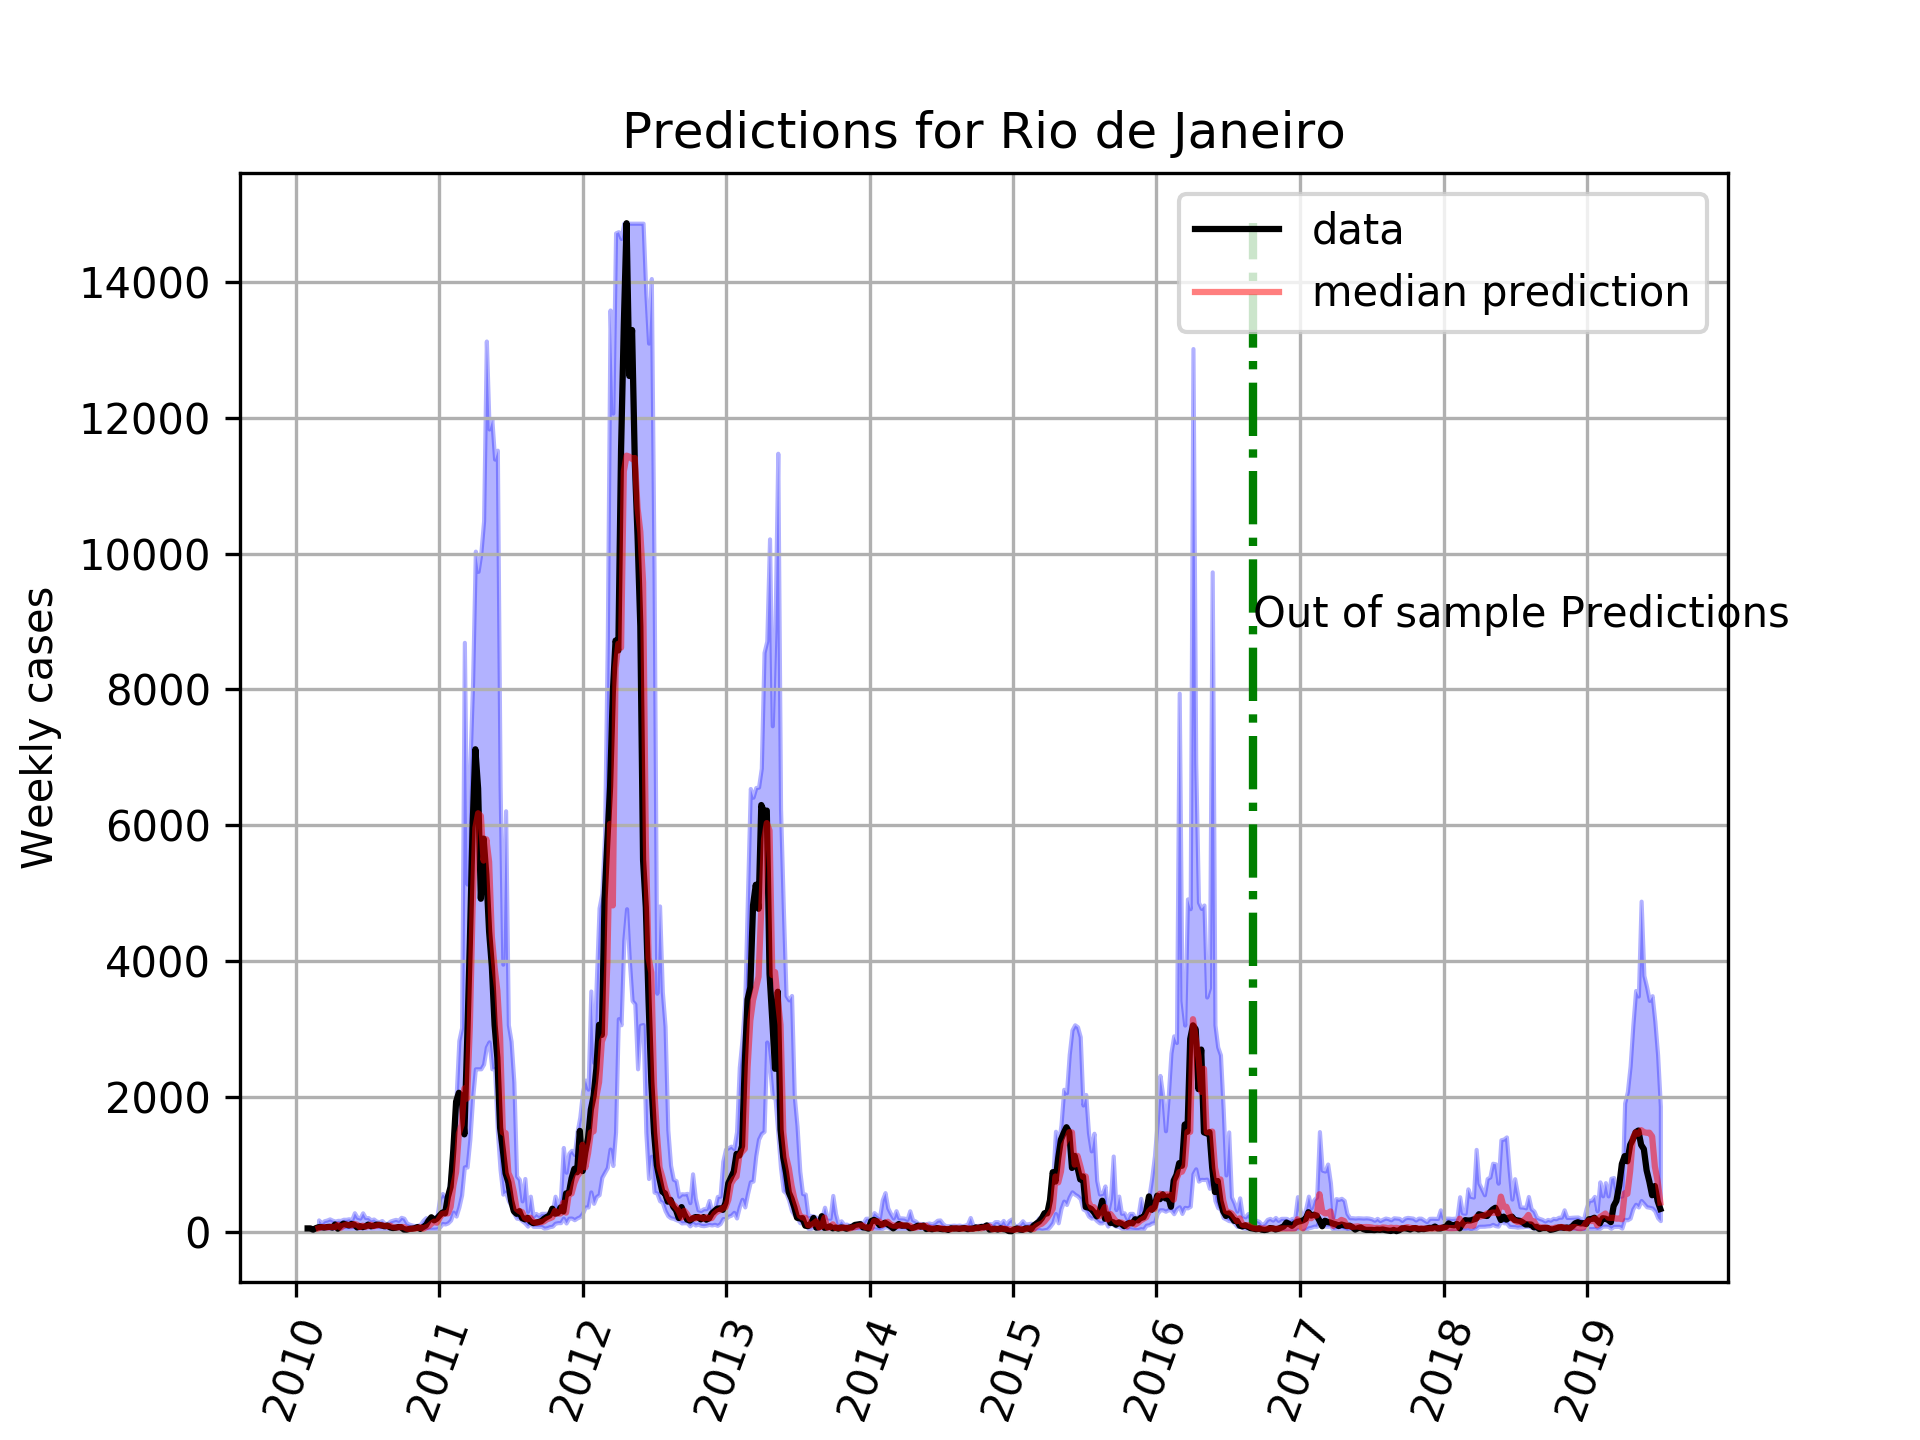
\includegraphics[width=0.8\linewidth]{figures/qf_Rio_de_Janeiro_dengue.png}
\captionof{figure}{\textbf{Baseline forecast for dengue in Rio de Janeiro.} 
Random quantile forest model trained on data from 2010 to mid 2016. Red line is 
the median prediction, with 95\% intervals in light 
purple.}\label{fig:dengue_RQF}
\end{center}%\vspace{1cm}

\section*{Results}
\noindent
Both models were fed available Chickungunya and Zika data, yielding 
reasonable predictions. Below are the forecasts for Chikungunya for the cities 
of Rio de Janeiro and Fortaleza.

\subsection*{RQF cross-predictions}
\begin{center}
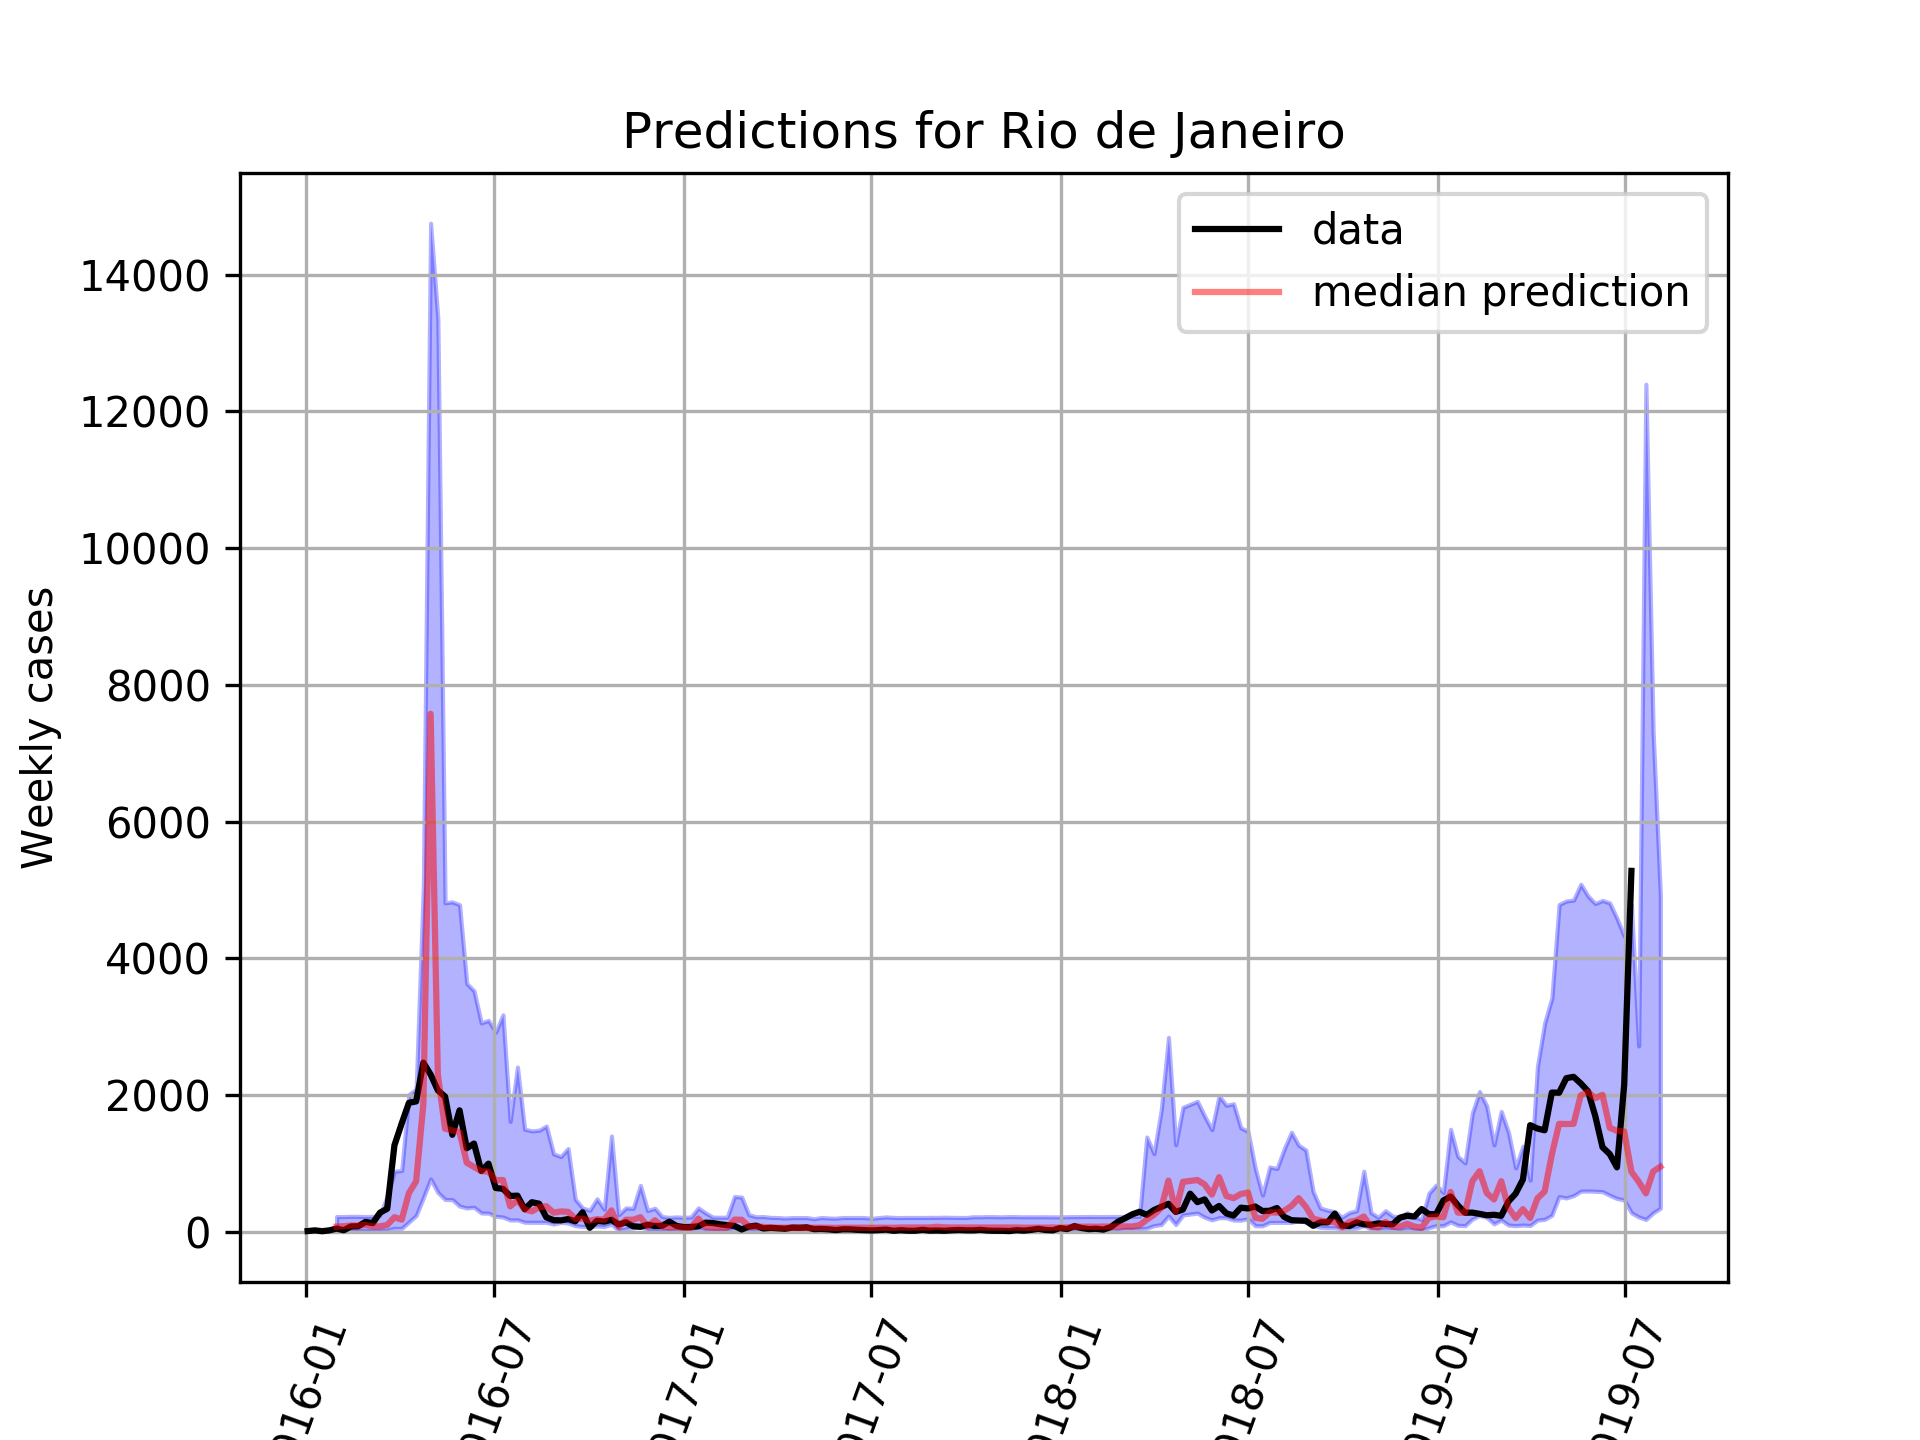
\includegraphics[width=0.8\linewidth]{figures/qf_chik_cross_Rio_de_Janeiro.png} 
\captionof{figure}{\textbf{Chikungunya forecasts based on dengue RQF model.} 
The 95\% confidence intervals are wider than those for dengue data, but include 
the observed data.}\label{fig:chik_rio_de_janeiro}
\end{center}%\vspace{1cm}

\begin{center}
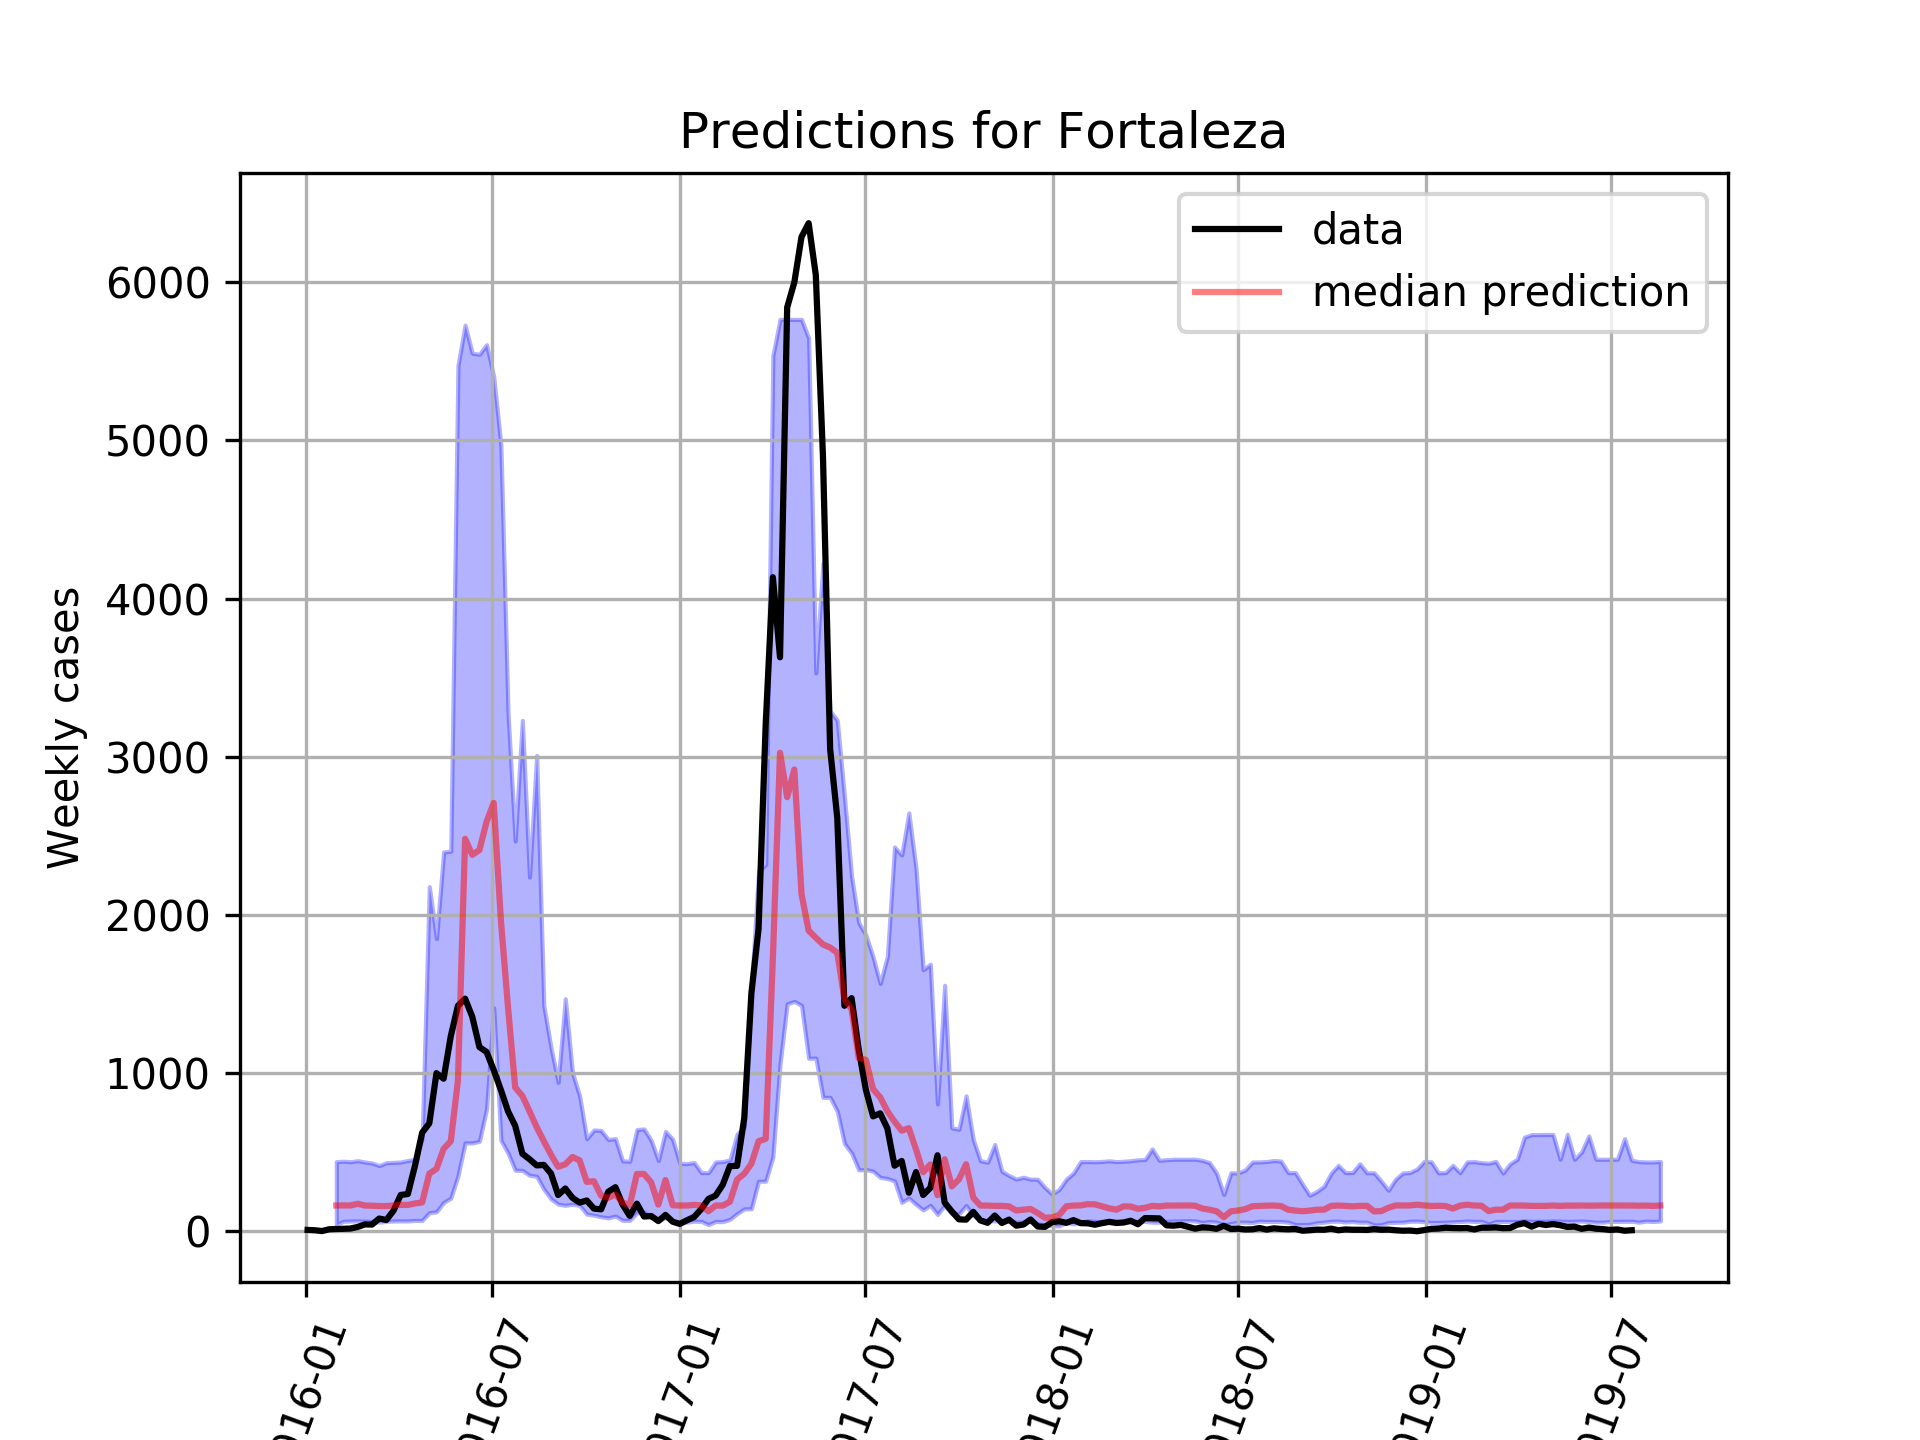
\includegraphics[width=0.8\linewidth]{figures/qf_chik_cross_Fortaleza.png} 
\captionof{figure}{\textbf{Chikungunya forecasts based on dengue RQF model.} 
The 95\% confidence intervals are wider than those for dengue data, but include 
the observed data.}\label{fig:chik_fortaleza}
\end{center}%\vspace{1cm}

Predictions where run from 2016 on since before this year Chikungunya and Zika 
did not circulate in Brazil. 

\begin{center}
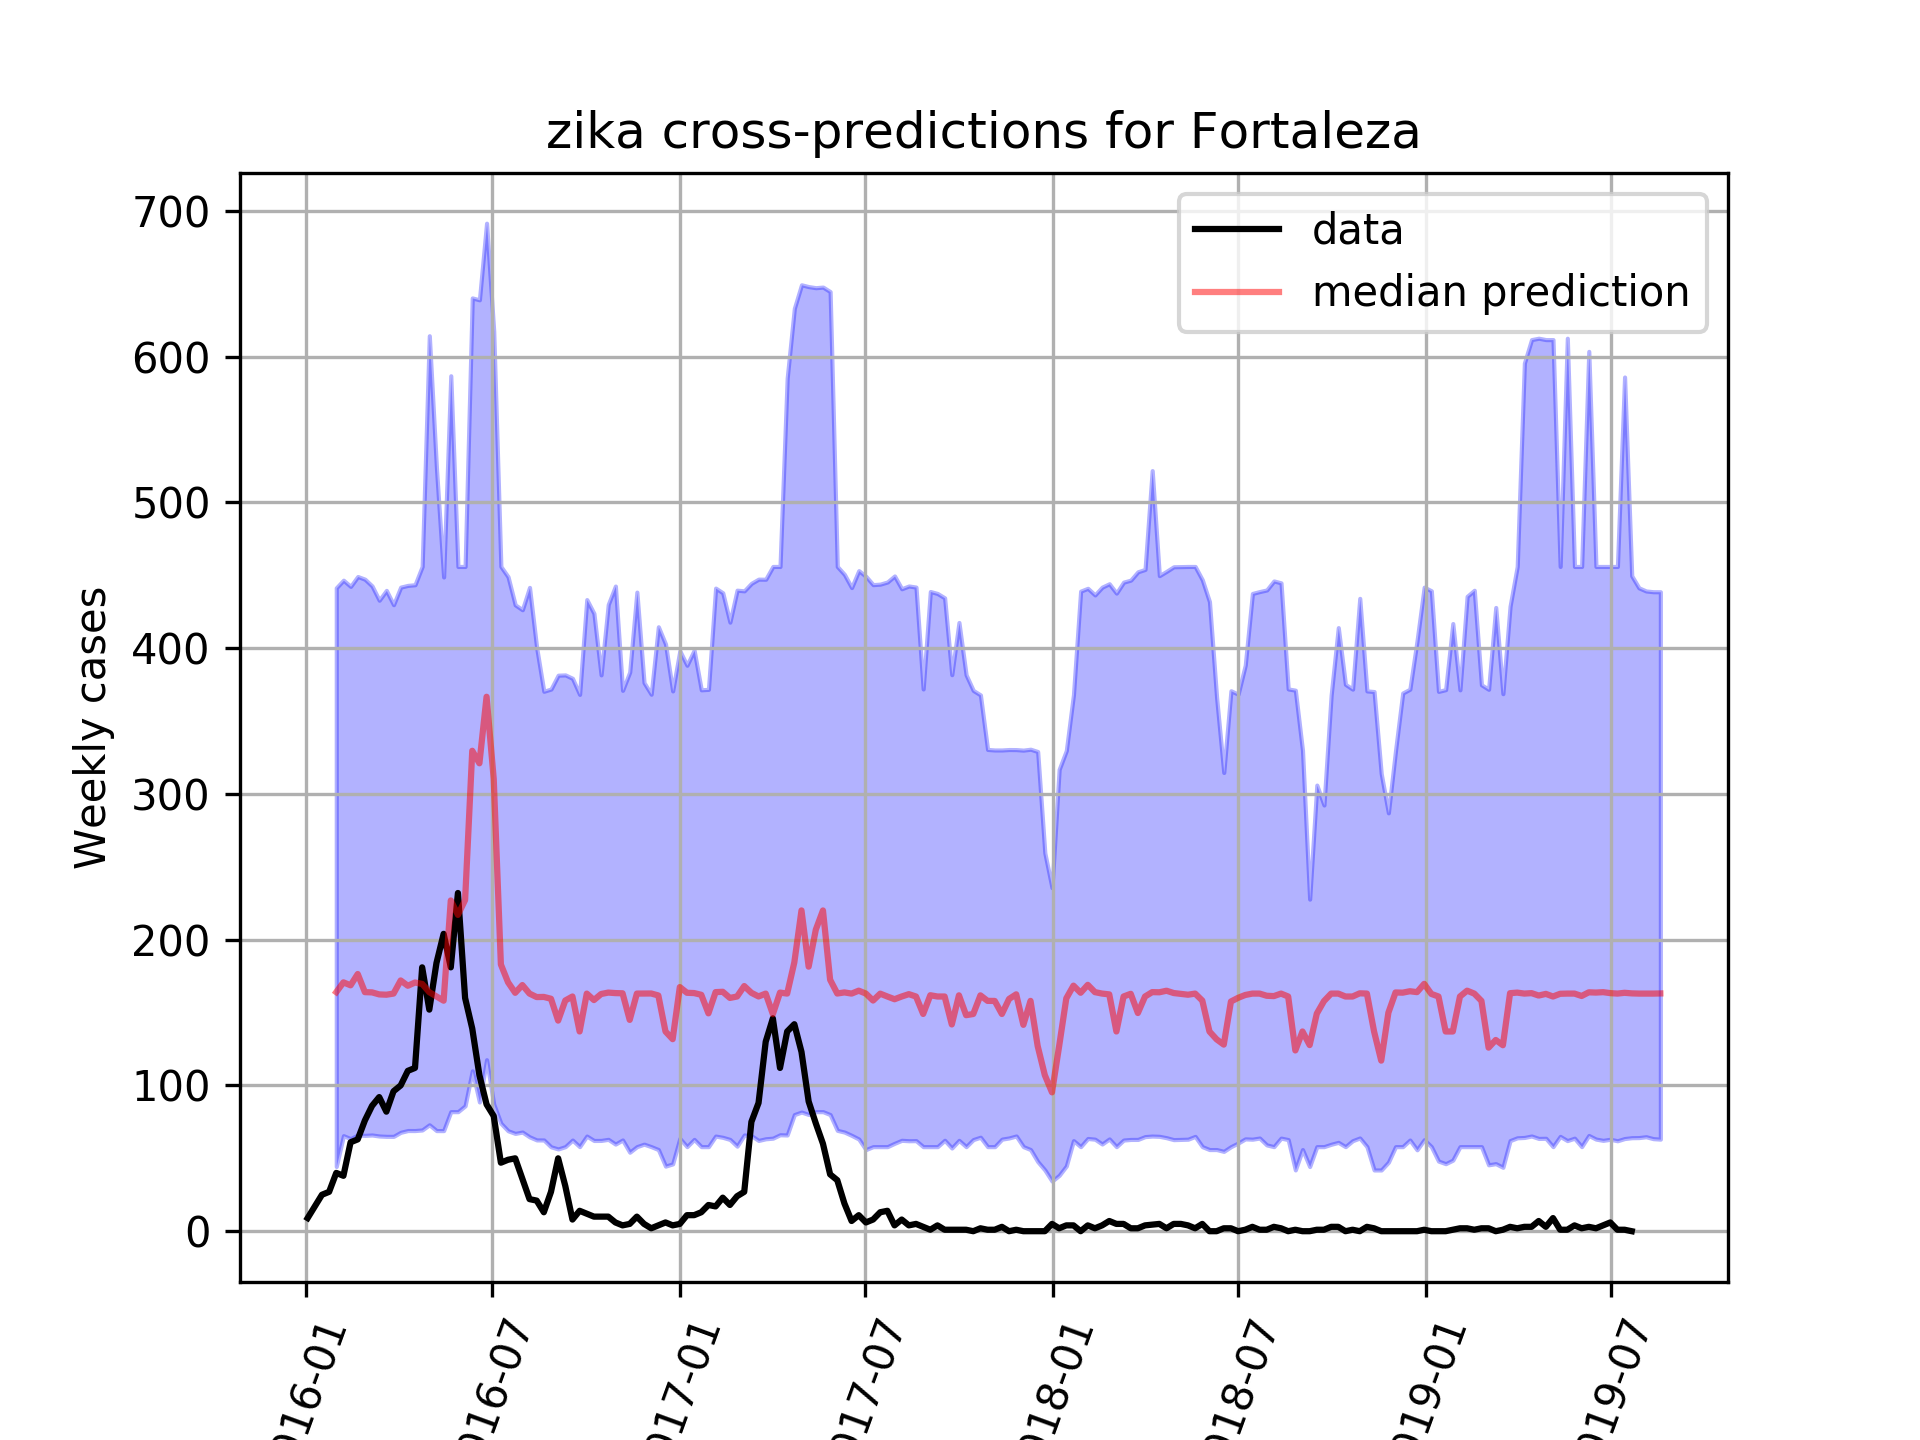
\includegraphics[width=0.8\linewidth]{figures/qf_zika_cross_Fortaleza}
\captionof{figure}{\textbf{Cross-predicting for Zika.} Zika forecasts based on 
dengue RQF, for the city of Fortaleza.}\label{fig:zika_fortaleza}
\end{center}

\subsection*{LSTM cross-predictions}

\begin{center}
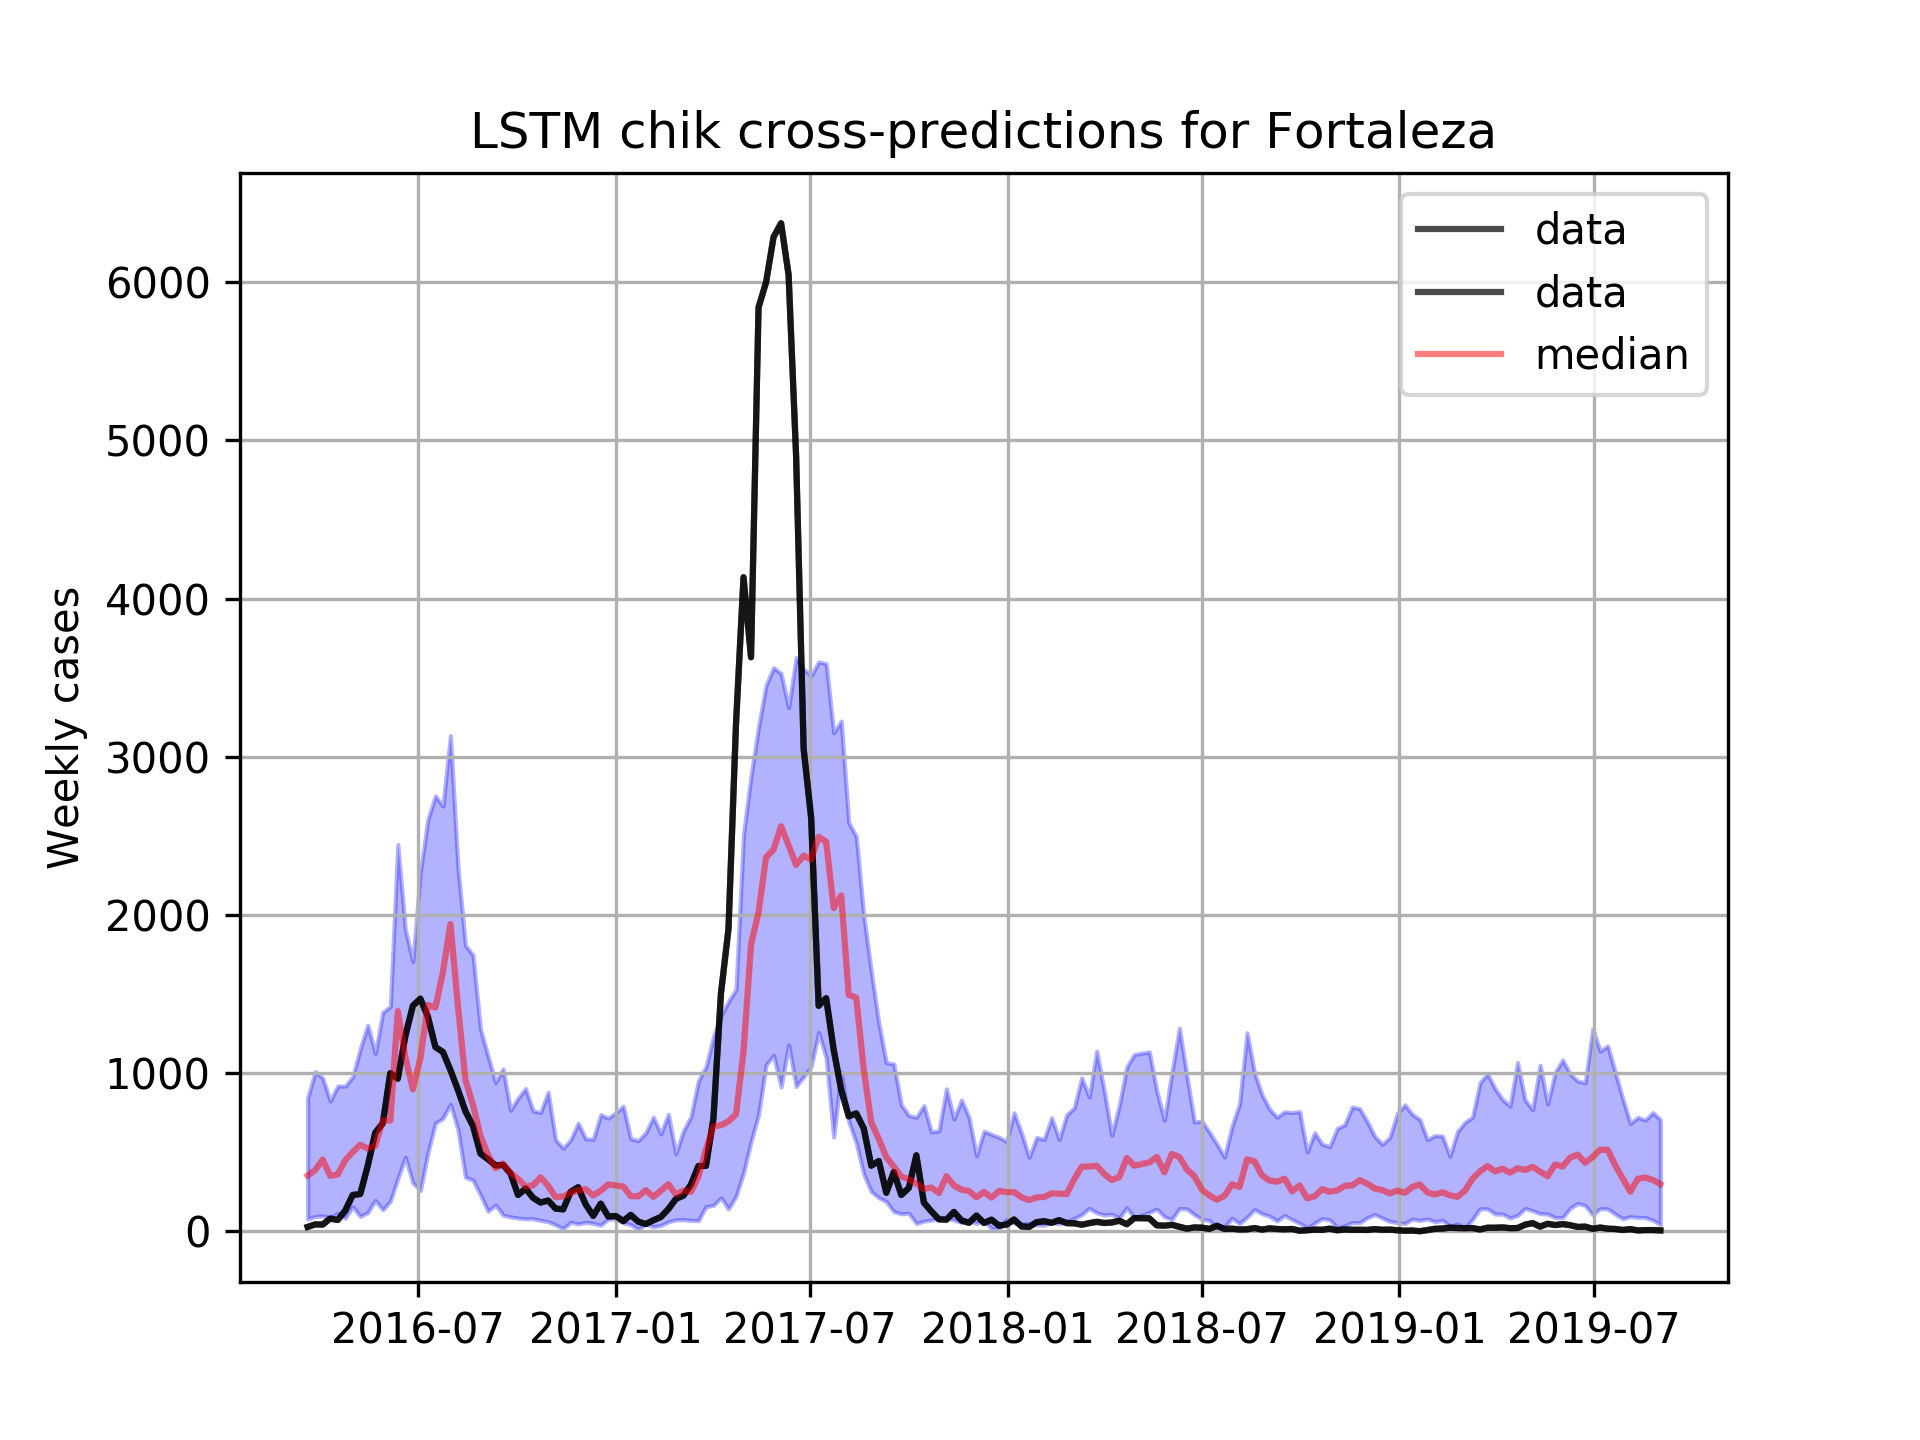
\includegraphics[width=0.8\linewidth]{figures/lstm_chik_cross_Fortaleza.png} 
\captionof{figure}{\textbf{Chikungunya forecasts based on dengue LSTM model.} 
The 95\% confidence intervals are wider than those for dengue data, but include 
the observed data.}\label{fig:lstm_chik_fortaleza}
\end{center}%\vspace{1cm}

\begin{center}
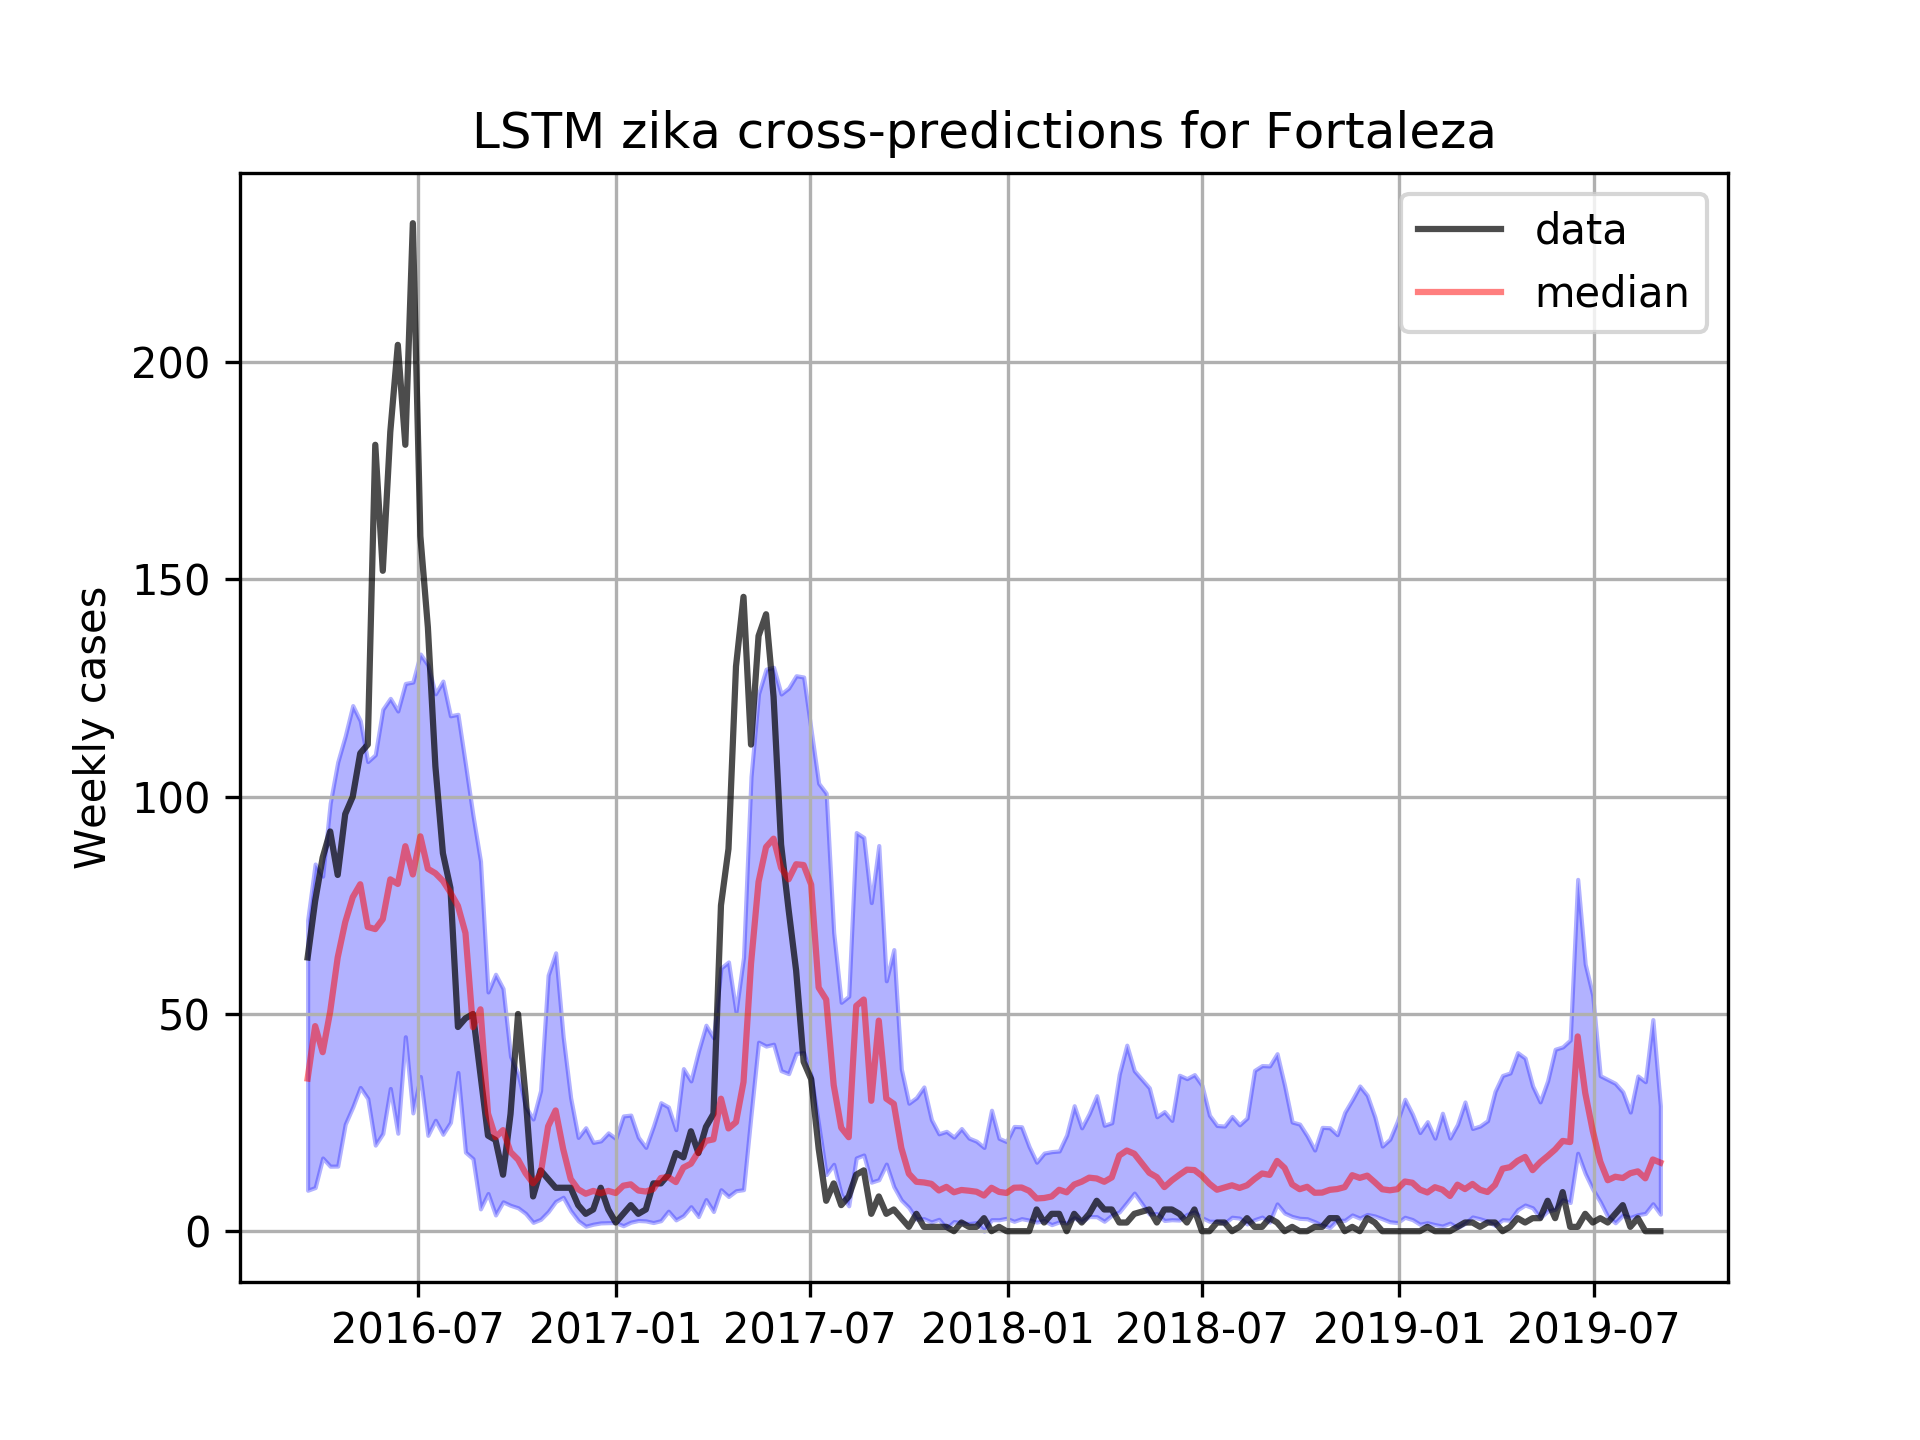
\includegraphics[width=0.8\linewidth]{figures/lstm_zika_cross_Fortaleza.png} 
\captionof{figure}{\textbf{Chikungunya forecasts based on dengue LSTM model.} 
The 95\% confidence intervals are wider than those for dengue data, but include 
the observed data.}\label{fig:lstm_chik_fortaleza}
\end{center}%\vspace{1cm}



\section*{Discussion}


\section*{Discussion and Conclusion}
Cross-disease forecasting models like the ones presented here are important 
because they allow us to take advantage from longer historic records from other 
diseases which share similar transmission mechanisms and environmental 
determinants.


The results presented here, expectedly show more uncertainty associated to 
cross-predictions when compared to forecasting the disease they were trained 
on. Nevertheless the models show reasonable accuracy when cross-predicting 
Chikungunya (figures \ref{fig:chik_rio_de_janeiro} and 
\ref{fig:chik_fortaleza}), perhaps more than the same models would be capable 
of 
if they were trained on the scarce available data for Chikungunya. 

For Zika, cross-predictions did not work as well (figure 
\ref{fig:zika_fortaleza}). Perhaps the fact that Zika can also be transmitted 
sexually\cite{coelho2016higher} makes its dynamic sufficiently different from 
dengue to make cross-predicting ineffective.

Machine learning models have shown great potential for infectious disease 
forecasting. However, long enough timeseries, essential to train such models 
are not easy to come by. In this work we have shown the potential of 
cross-disease forecasts, for diseases with similar transmission mechanisms. 
Despite the encouraging initial results there is still plenty of room for 
improvements of such models. 

Supplementary figures with results for many other brazilian cities are 
available from this github repository: \url{github.com/AlertaDengue/Geomed_2019}

%----------------------------------------------------------------------------------------
%	References
%----------------------------------------------------------------------------------------

\small
\nocite{*} % Print all references regardless of whether they were cited in the poster or not
\bibliographystyle{plain} % Plain referencing style
\bibliography{sample} % Use the example bibliography file sample.bib


%----------------------------------------------------------------------------------------
%	Funding
%----------------------------------------------------------------------------------------
\section*{Funded by}
\begin{center}\vspace{0cm}

\includegraphics[width=0.65\linewidth]{figures/fundedby.png}
\end{center}%\vspace{1cm}

%----------------------------------------------------------------------------------------

\end{multicols}
\end{document}
